\chapter{System Architecture Overview}



This chapter presents the overall system architecture organised into three functional tiers. The three-tier decomposition enables independent development, testing, and scaling of each component. Figure~\ref{fig:arch} presents the complete end-to-end pipeline from sensor capture to dashboard visualisation.

\begin{figure}[htbp]
    \centering
    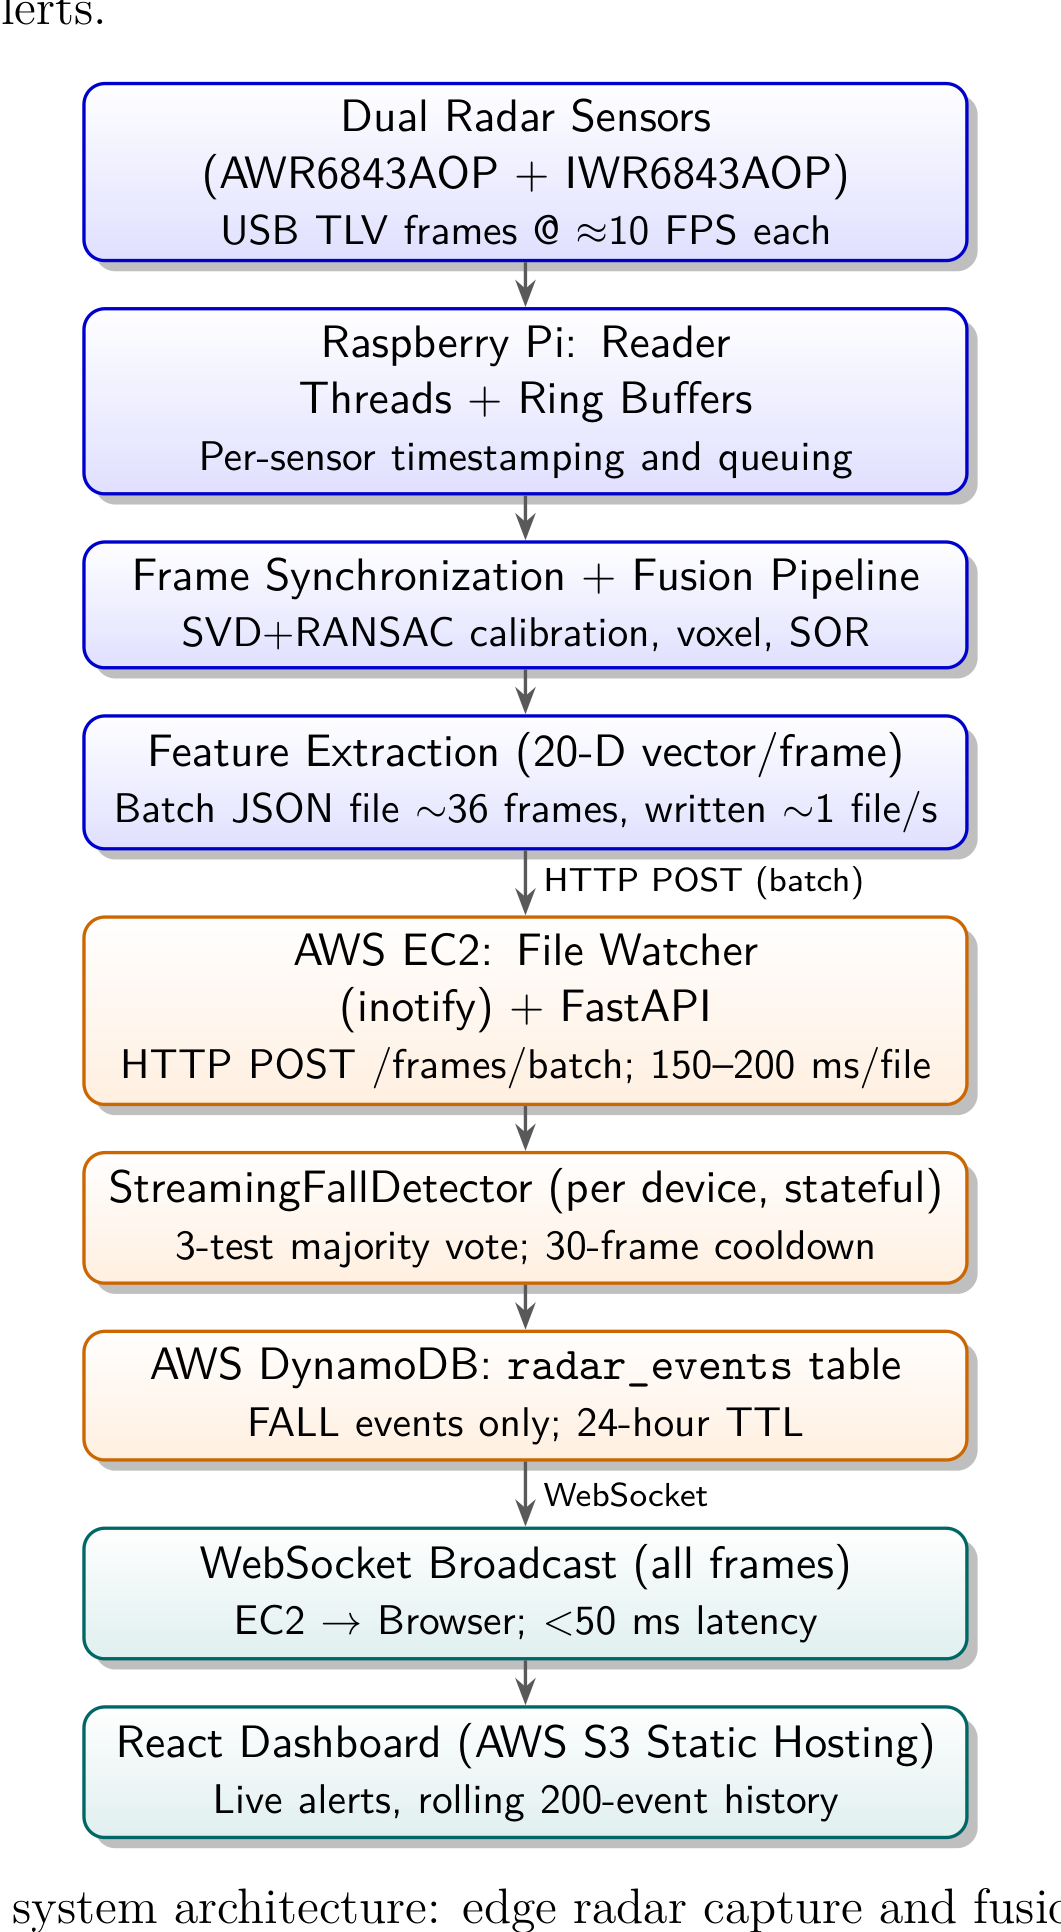
\includegraphics[width=\textwidth,height=0.8\textheight,keepaspectratio]{Figures/flowchart_p14.png}
    \caption{End-to-end system architecture}
    \label{fig:arch}
\end{figure}

 

\section{Three-Tier Architecture}

\textbf{1. Edge Tier (Raspberry Pi):} Two radar sensors deliver raw TLV frames over USB. A dedicated reader thread per sensor timestamps and buffers each frame. A pairing thread synchronises frames across both sensors, drives the auto-calibration and fusion pipeline, extracts a 20-dimensional feature vector per frame, and batches \textit{$\sim$}36 frames into a single JSON file written to a local watch directory approximately once per second.

\textbf{2. Cloud Inference Tier (AWS EC2):} A file watcher detects each new batch file via Linux inotify and POSTs the full batch to a FastAPI service running inside a Docker container on AWS EC2 (region \texttt{ap-south-1}, Mumbai). The API applies a stateful, rule-based fall detector per device, persists confirmed fall events to AWS DynamoDB with a 24-hour TTL, and broadcasts every inference result to connected dashboard clients via WebSocket.

\textbf{3. Presentation Tier (AWS S3 + Browser):} A React single-page application hosted on AWS S3 static website hosting connects to the WebSocket endpoint on page load, maintains a rolling buffer of 200 recent events, and renders live activity metrics and fall alerts.


\section{Inter-Tier Communication Protocols}

Between the edge tier and cloud tier, communication occurs via HTTP POST requests carrying JSON-encoded batch files. The use of stateless HTTP rather than a persistent TCP connection simplifies retry logic: if a POST fails due to transient network interruption, the edge device can re-attempt without any server-side state synchronisation.

Between the cloud tier and the presentation tier, communication occurs via a persistent WebSocket connection, providing server-push capability for immediate alert delivery.

WebSocket is chosen over periodic HTTP polling because it eliminates polling latency and allows the server to push each inference result to the browser the instant it is produced, essential for achieving sub-400 ms end-to-end latency.

\section{Containerisation and Deployment}

The FastAPI application on EC2 is packaged inside a Docker container, providing environment reproducibility and simplifying deployment. Nginx acts as a reverse proxy in front of Uvicorn, handling TLS termination and WebSocket upgrade negotiation. The Docker-based deployment ensures the cloud inference stack can be reproduced identically on any EC2 instance type with minimal configuration changes, and simplifies blue-green deployment for updates.


\section{Amazon Web Services (AWS) Infrastructure}

This project relies on three core AWS services --- EC2, DynamoDB, and S3 --- each selected for its unique properties in the context of real-time, serverless-friendly, event-driven radar inference.

\subsection{AWS Overview}

Amazon Web Services (AWS) is the world's most comprehensive and broadly adopted cloud platform, offering over 200 fully featured services from data centres globally. AWS enables organisations to lower costs, become more agile, and innovate faster by removing the need to own and maintain physical infrastructure. The key characteristics of AWS relevant to this project are:

\begin{itemize}
    \item \textbf{Global Regions and Availability Zones:} AWS infrastructure is divided into geographic Regions, each containing multiple isolated Availability Zones (AZs). This project uses the \texttt{ap-south-1} (Mumbai) Region, chosen for minimal round-trip latency to the edge device located in India.
    \item \textbf{Pay-as-you-go Pricing:} Resources are billed only for actual usage, making prototyping cost-efficient.
    \item \textbf{Managed Services:} AWS abstracts operating-system-level administration for services like DynamoDB and S3, eliminating patching, scaling, and backup overhead.
    \item \textbf{Security and IAM:} AWS Identity and Access Management (IAM) provides fine-grained, role-based access control. The EC2 instance is assigned an IAM role granting least-privilege access to only the \texttt{radar\_events} DynamoDB table, following the principle of least privilege.
\end{itemize}

\subsection{AWS EC2 --- Elastic Compute Cloud}

\textbf{Service Description:} Amazon Elastic Compute Cloud (EC2) provides resizable virtual machine instances in the cloud. An EC2 instance is a virtual server with a configurable combination of CPU, memory, storage, and networking capacity. Instances are launched from \textit{Amazon Machine Images} (AMIs), which bundle the operating system and pre-installed software.

\textbf{Role in this Project:} EC2 hosts the cloud inference tier. Specifically:

\begin{itemize}
    \item A \textbf{t3.micro} instance (2 vCPU, 1 GB RAM) running Amazon Linux 2 is deployed in the \texttt{ap-south-1} (Mumbai) Region. This instance type is sufficient because the rule-based \textit{StreamingFallDetector} executes in under 1 ms per frame, leaving ample headroom.
    \item The FastAPI application (\texttt{radar-api-main.py}) is containerised using \textbf{Docker} and served by \textbf{Uvicorn} (ASGI server) behind \textbf{Nginx} (reverse proxy). Nginx handles port 80 traffic, WebSocket upgrade headers, and distributes requests to Uvicorn.
    \item An \textbf{Elastic IP address} is assigned to the instance, providing a static public IP that survives instance stop/start cycles. The IP \texttt{43.205.167.81} is the publicly reachable endpoint used by the Raspberry Pi and the React dashboard.
    \item \textbf{Security Groups} (virtual firewalls) restrict inbound traffic to only port 80 (HTTP/WebSocket) and port 22 (SSH for administration), rejecting all other traffic.
\end{itemize}

\textbf{Key EC2 Features Utilised:}

\begin{itemize}
    \item \textbf{Elastic IP:} A static public IPv4 address that does not change across reboots, ensuring the Raspberry Pi and browser always reach the same endpoint without DNS configuration.
    \item \textbf{Security Groups:} Stateful firewall rules at the instance level. Inbound rules allow TCP/80 from \texttt{0.0.0.0/0} (any IP) for the API and WebSocket, and TCP/22 from the developer's IP for SSH.
    \item \textbf{IAM Instance Profile:} Grants the EC2 process permission to call \texttt{dynamodb:PutItem} and \texttt{dynamodb:Query} on the \texttt{radar\_events} table without embedding credentials in the application code.
    \item \textbf{User Data Script:} A startup script installs Docker, pulls the application image, and launches the container on every boot, enabling fully automated re-provisioning.
    \item \textbf{CloudWatch Logs:} Uvicorn application logs are streamed to AWS CloudWatch, enabling remote log inspection without SSH access.
\end{itemize}

\subsection{AWS DynamoDB --- NoSQL Event Store}

\textbf{Service Description:} Amazon DynamoDB is a fully managed, serverless, key-value and document NoSQL database that delivers single-digit millisecond performance at any scale. It requires no capacity planning for reads/writes below the provisioned throughput threshold and provides built-in high availability by replicating data across three Availability Zones within a Region.

\textbf{Role in this Project:} DynamoDB serves as the persistent event log for confirmed fall events:

\begin{itemize}
    \item \textbf{Table name:} \texttt{radar\_events}
    \item \textbf{Partition key:} \texttt{device\_id} (String) --- uniquely identifies each radar node (e.g.\ \texttt{rpi-1}).
    \item \textbf{Sort key:} \texttt{ts} (String, ISO 8601 UTC) --- enables time-ordered queries within a device's event history.
    \item \textbf{Global Secondary Index:} A \texttt{pk} attribute (always set to \texttt{"all"}) allows scanning across all devices when a unified event feed is required.
    \item \textbf{TTL (Time to Live):} Each item carries an \texttt{expire\_at} attribute set to 24 hours after insertion. DynamoDB's TTL feature automatically deletes expired items, preventing unbounded table growth and eliminating the need for a scheduled purge job.
    \item \textbf{Write path:} Only \texttt{FALL}-classified frames trigger a \texttt{PutItem} call, keeping write throughput low (typically $<$1 write per minute per device under normal conditions).
    \item \textbf{Read path:} The \texttt{GET /history} endpoint issues a \texttt{Query} using the \texttt{device\_id} partition key with \texttt{ScanIndexForward=False} to retrieve the most recent events in descending timestamp order.
\end{itemize}

\textbf{Rationale for DynamoDB over alternatives:}

\begin{itemize}
    \item \textbf{Schema-free:} No migration required when new debug fields (e.g.\ \texttt{z\_drop}, \texttt{drop\_streak}) are added to the fall event record.
    \item \textbf{Built-in TTL:} Automatic data expiry without a cron job or Lambda function.
    \item \textbf{Horizontal scalability:} Write throughput scales with additional radar nodes without database reconfiguration.
    \item \textbf{Single-digit millisecond writes:} The \texttt{PutItem} call completes in approximately 30 ms (Table~\ref{tab:latency_budget}) --- entirely within the 400 ms system latency budget.
\end{itemize}

\subsection{AWS S3 --- Static Website Hosting for the React Dashboard}

\textbf{Service Description:} Amazon Simple Storage Service (S3) is an object storage service offering industry-leading scalability, data availability (99.999999999\% durability), security, and performance. S3 stores objects (files) inside \textit{buckets}. One of its built-in features is \textbf{Static Website Hosting}, which serves the contents of a bucket as a public website without requiring a web server.

\textbf{Role in this Project:} The React single-page application (SPA) is compiled into a set of static HTML, CSS, and JavaScript files and uploaded to an S3 bucket configured for static website hosting. Key configuration details:

\begin{itemize}
    \item \textbf{Bucket name:} \texttt{radar-dashboard} (or similar, in \texttt{ap-south-1}).
    \item \textbf{Static Website Hosting:} Enabled with \texttt{index.html} as both the index document and the error document (required for client-side routing).
    \item \textbf{Bucket Policy:} A public-read bucket policy grants \texttt{s3:GetObject} to any principal (\texttt{"Principal": "*"}), making all files publicly accessible.
    \item \textbf{CORS Configuration:} A Cross-Origin Resource Sharing (CORS) rule allows the browser served from the S3 URL to open a WebSocket connection to the EC2 instance at a different origin.
\end{itemize}

\textbf{Dashboard Behaviour:} On page load, the React application:
\begin{enumerate}
    \item Issues a \texttt{GET /history?device\_id=rpi-1\&limit=60} REST call to the EC2 API to pre-populate the inference history panel with recent fall events stored in DynamoDB.
    \item Opens a persistent WebSocket connection to \texttt{ws://<EC2-IP>/ws}.
    \item Renders incoming JSON messages as live inference cards in real time.
    \item On a \texttt{"FALL"} event, switches the UI to an alert state with a prominent visual indicator.
\end{enumerate}

\textbf{Rationale for S3 Static Hosting over alternatives (e.g.\ EC2-served React):}
\begin{itemize}
    \item \textbf{Zero server maintenance:} No web server process to manage, patch, or monitor.
    \item \textbf{99.99\% availability SLA:} S3 static hosting provides higher availability than a single EC2 instance.
    \item \textbf{Global edge delivery:} S3 can be paired with CloudFront (AWS CDN) for low-latency global delivery with a single configuration change.
    \item \textbf{Cost:} Static file hosting costs only storage (\textasciitilde\$0.023/GB-month) and data transfer, an order of magnitude cheaper than running a web server on EC2 24/7.
\end{itemize}

\subsection{Docker and Nginx on EC2}

\textbf{Docker:} The FastAPI application and all its Python dependencies (NumPy, boto3, FastAPI, Uvicorn, Pydantic) are packaged into a Docker image. This ensures that the runtime environment is identical on any EC2 instance type, eliminating ``works on my machine'' configuration drift. The \texttt{Dockerfile} specifies a slim Python 3.11 base image, installs dependencies from \texttt{requirements.txt}, and sets the Uvicorn entry point.

\textbf{Nginx as Reverse Proxy:} Nginx listens on port 80 and forwards HTTP requests to Uvicorn (listening on \texttt{127.0.0.1:8000}). The Nginx configuration includes:
\begin{itemize}
    \item \textbf{WebSocket proxying:} \texttt{proxy\_set\_header Upgrade \$http\_upgrade} and \texttt{proxy\_set\_header Connection "upgrade"} headers instruct Nginx to upgrade HTTP/1.1 connections to WebSocket without dropping the persistent connection.
    \item \textbf{Buffering disabled:} \texttt{proxy\_buffering off} ensures WebSocket frames are forwarded immediately without accumulation delay.
    \item \textbf{Read timeout extension:} \texttt{proxy\_read\_timeout 3600s} keeps idle WebSocket connections alive for up to one hour without Nginx closing them.
\end{itemize}

\subsection{Summary of AWS Services Used}

Table~\ref{tab:aws_summary} summarises all AWS services utilised in this project, their roles, and the key configuration parameters.

\begin{table}[H]
\caption{AWS Services Used in the Radar Fall Detection System}
\label{tab:aws_summary}
\centering
\begin{tabularx}{\textwidth}{@{} l X X @{}}
\toprule
\textbf{Service} & \textbf{Role} & \textbf{Key Configuration} \\ \midrule
EC2 (t3.micro) & Cloud inference host; FastAPI + Docker & Region: ap-south-1; Elastic IP; Security Group TCP/80, TCP/22 \\
DynamoDB & Persistent fall event log & Table: radar\_events; PK: device\_id; SK: ts; TTL: 24 h \\
S3 Static Hosting & React dashboard delivery & Public bucket; index.html; CORS enabled \\
IAM & Least-privilege access control & Instance role: PutItem + Query on radar\_events only \\
CloudWatch & Application log aggregation & Uvicorn stdout/stderr streamed to log group \\ \bottomrule
\end{tabularx}
\end{table}